% multiple1902 <multiple1902@gmail.com>
% available on https://code.google.com/p/xjtu-cs-lect/
% licensed under cc by-sa 3.0
\documentclass[12pt,openany,twoside]{book}
\usepackage{amsthm,amssymb,fullpage}
\usepackage[slantfont,boldfont,CJKnumber,CJKtextspaces,CJKmathspaces]{xeCJK}
\usepackage{tabularx}
\usepackage{graphicx}
\usepackage{booktabs}
\usepackage{multicol}
\usepackage{pstricks}
\usepackage{pst-node}
\usepackage{pst-blur}
\usepackage{rotating}
\usepackage[
    pdftitle={西安交通大学计算机系课堂笔记 http://code.google.com/p/xjtu-cs-lect/}
]{hyperref}
\setCJKmainfont{細明體}
\setCJKsansfont{微軟正黑體}

\makeatletter
\renewcommand\section{\@startsection{section}{1}{\z@}%
{-3.5ex \@plus -1ex \@minus -.2ex}%
{2.3ex \@plus.2ex}%
{\Large \sf}}
\renewcommand\subsection{\@startsection {subsection}{2}{\z@}%
{-3.25ex\@plus -1ex \@minus -.2ex}{1.5ex \@plus .2ex}%
{\normalfont \large \sf}}
\renewcommand\subsubsection{\@startsection {subsubsection}{3}{\z@ }{-3.25ex\@plus -1ex \@minus -.2ex}{1.5ex \@plus .2ex}{\normalfont \normalsize \sf }}
\renewcommand\chapter{
\if@openright \cleardoublepage \else \clearpage \fi \thispagestyle {plain}\global \@topnum \z@ \@afterindentfalse \secdef \@chapter \@schapter
}
\renewcommand\paragraph{
\@startsection {paragraph}{4}{\z@ }{3.25ex \@plus 1ex \@minus .2ex}{-1em}{\normalfont \normalsize \sf }
}
\renewcommand\subparagraph{
\@startsection {subparagraph}{5}{\parindent }{3.25ex \@plus 1ex \@minus .2ex}
{-1em}{\normalfont \normalsize \sf  }
}
\makeatother

\def\d{\mathrm{d}}
\def\e{\mathrm{e}}
\renewcommand{\tablename}{表} 
\renewcommand{\figurename}{图} 

\setlength\parindent{2em}

\hypersetup{
    colorlinks,%linkcolor=blue,anchorcolor=blue,citecolor=green,
    pdfcreator={TeX}, 
    pdfauthor={multiple1902@gmail.com}
    }

\title{\sf \Huge \bf 刘国荣组合数学课程笔记\thanks{\rm 基于课堂笔记整理, 依据课件和更多资料修正和补充. 授课教师: 刘国荣}}
\author{戴唯思\quad 张潇}
\begin{document}

\graphicspath{comb_notes/}

\clearpage

\sf \Large

西安交通大学计算机系课堂笔记

\url{http://code.google.com/p/xjtu-cs-lect/}

\vskip 1cm

以GNU GPL v2释出: \url{https://www.gnu.org/licenses/gpl-2.0.txt}

\rm \normalsize
\thispagestyle{empty}
\setcounter{page}{0}
\clearpage


\maketitle

% multiple1902 <multiple1902@gmail.com>
% available on https://code.google.com/p/xjtu-cs-lect/
% licensed under cc by-sa 3.0
\setcounter{chapter}{-1}
\chapter{绪论}

\section{什么是组合数学}

    \textsf{组合数学}(combinatorial mathematics)是研究离散结构的存在, 计数, 分析和优化等问题的一门学科. 它

    \begin{itemize}
        \item (构造性)研究事物在给定模式下的配置(也称为方案),
        \item (存在性)研究这种配置(方案)是否存在
            \begin{itemize}
                \item 所有可能配置(方案)的数目和分类(计数),
                \item 配置(方案)的各种性质(优化).
            \end{itemize}
    \end{itemize}

\section{古代组合数学}

    组合数学源远流长, 但在远古时代这类问题往往联系着数的神秘主义出现. 

    \subsection{河图, 洛书}

        河图洛书, 来自上古时代有关数字排列之图案. 在宋朝之前, 洛书的记述只有文字, 一直到陈抟, 才提出了洛书的图案. 有人认为是重要的中国传统易理哲学部分, 后被广泛应用于风水、占卜等术数中. 
       
        \begin{figure}[!h]
            \centering
            \begin{minipage}[t]{.4\linewidth}
                \centering
                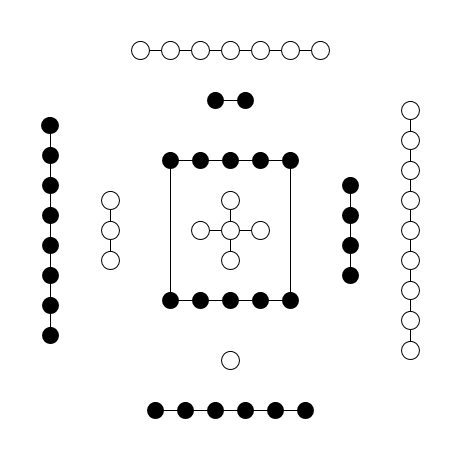
\includegraphics[width=.8\linewidth]{comb_notes/chap0_inc/河图.png}
                    % public domain
                \caption{河图}
                \label{fig:0:hetu}
            \end{minipage}
            \begin{minipage}[t]{.4\linewidth}
                \centering
                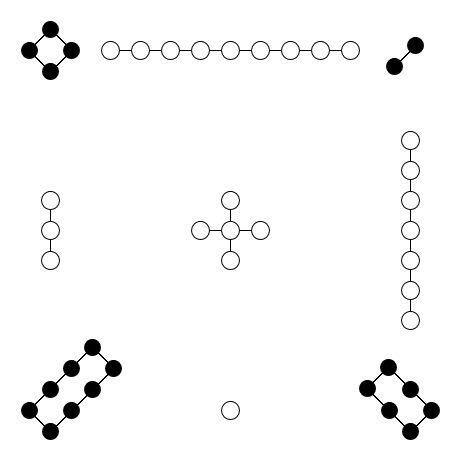
\includegraphics[width=.8\linewidth]{comb_notes/chap0_inc/洛书.png}
                    % public domain
                \caption{洛书}
                \label{fig:0:luoshu}
            \end{minipage}
        \end{figure}

        今人有人认为《河图》(图\ref{fig:0:hetu})是银河系双螺旋结构的数理模型.

        《洛书》实际上是一三阶幻方: \textsf{幻方}是每行、每列、主副对角线上数字之和全相等的方阵. $n$阶幻方的\textsf{幻和}$S_n=\frac{n(n^2+1)}{2}$

        \subsubsection{奇数阶幻方的构造}

            \paragraph{劳伯尔算法}

                \begin{enumerate}
                    \item 在顶行(即第一行)中间写上数1,
                    \item 下一个数填写在前一个数的右上角位置上,
                    \item 当右上角不存在或已被填写时, 按下述规则修改之:
                        \begin{enumerate}
                            \item 当到达顶行时, 认为底行(即第$n$行)接在顶行之上;
                            \item 当到达最右列(即第$n$列)时, 认为最左列(即第一列)接在最右列之右;
                            \item 当欲填位置上已被填写, 或达到顶行最右列(即右上角)时, 下一个数填在前一个数的下边.
                        \end{enumerate}
                \end{enumerate}

            \paragraph{麦哲里克算法}

                \begin{enumerate}
                    \item 先在正中央方格的上方写上数1,
                    \setcounter{enumi}{2}
                    \item 
                        \begin{enumerate}
                            \setcounter{enumii}{2}
                            \item 当欲填位置上已被填写,或达到顶行最右列(即右上角)时,下一个数填在前一个数的上方两格处.
                        \end{enumerate}
                \end{enumerate}

% multiple1902 <multiple1902@gmail.com>
% available on https://code.google.com/p/xjtu-cs-lect/
% licensed under cc by-sa 3.0
\chapter{排列与组合}

\section*{课前思考}

    \begin{enumerate}
        \item 2个互异的球放入3个互异的盒子, 每个盒子至多一个球, 有多少方案? 
        \item 2个互异的球放入3个互异的盒子, 每个盒子球数不限, 有多少方案? 
        \item 2个相同的球放入3个互异的盒子, 每个盒子至多一个球, 有多少方案? 
        \item 3个人围成一圈, 有多少方案? 
        \item 3颗不同的珠子串成一串项链, 有多少方案? 
        \item 5个人(每人都会开车)分乘2辆小轿车(每车4座), 有多少方案? 
    \end{enumerate}

\section{加法原理与乘法原理}

    \paragraph{加法原理}
        
        设事件$A_1$有$m_1$种产生方式, 事件$A_2$有$m_2$种产生方式, \ldots, 事件$A_n$有$m_n$种产生方式, 则事件$A_1$或$A_2$或$\ldots$或$A_n$之一有$m_1+m_2+\cdots+m_n$种产生方式.

        \subparagraph{集合论语言}

            若$|A_1|=m_1, |A_2|=m_2, \cdots, |A_n|=m_n$, 并且$A_i\cap A_j=\emptyset(1\leqslant i\neq j\leqslant n)$, 则$|A_1\cup A_2\cup\cdots\cup A_n|=m_1+m_2+\cdots+m_n$.

    \paragraph{乘法原理}

        设事件$A_1$有$m_1$种产生方式, 事件$A_2$有$m_2$种产生方式, \ldots, 事件$A_n$有$m_n$种产生方式, 则事件$A_1$与$A_2$与$\ldots$与$A_n$之一有$m_1\times m_2\times \cdots\times m_n$种产生方式.

        \subparagraph{集合论语言}

            若$|A_1|=m_1, |A_2|=m_2, \cdots, |A_n|=m_n$, 并且$A_1\times A_2\times \cdots \times A_n=\{(a_1,a_2,\cdots,a_n)|a_i\in A_i(1\leqslant i\leqslant n)\}$, 则$|A_1\times A_2\times\cdots\times A_n|=m_1+m_2+\cdots+m_n$.

\section{排列与组合}

    \subsection{无重排列}

        \begin{definition}[无重排列]
            从$n$个不同的元素中, 取$r$个不重复的元素, 按次序排成一列, 称为从$n$个元中取$r$个元的\textsf{(无重)排列}. 这些排列的全体组成的集合用$P(n,r)$表示. 排列的个数用$P(n,r)$表示. 当$r=n$时, 称为\textsf{全排列}. 一个排列也可看作一个字符串, $r$也称为排列或字符串的长度. 
        \end{definition}

        \begin{caution}
            一般没说可重复意即无重复
        \end{caution}

        \begin{theorem}
            $P(n,r)=n(n-1)\cdots(n-r+1)=\frac{n!}{(n-r)!}$
        \end{theorem}

    \subsection{无重组合}

        \begin{definition}[无重组合]
            从$n$个不同元素中, 取$r$个不重复的元素, 不考虑其次序, 构成一个子集, 称为从$n$个元中取$r$个元的\textsf{(无重)组合}. 这些组合的全体组成的集合用$\mathbf{C(n,r)}$表示, 组合的个数用$C(n,r)$或$n\choose r$表示.
        \end{definition}
        \begin{theorem}
            $C(n,r)=\frac{n!}{r!(n-r)!}$
        \end{theorem}

        \subparagraph{组合模型}

            组合的计数相当于将$r$个相同的球放入$n$个不同的盒子里, 每盒最多1个球的方案数.

    \subsection{可重排列}

        \begin{definition}[可重排列]
            从$n$个不同的元素中, 取$r$个可重复的元素, 按次序排成一列, 称为从$n$个元中取$r$个元的\textsf{可重排列}. 这些排列的全体组成的集合, 用$\mathbf{\overline{P}(n,r)}$表示.  排列的个数用$\overline{P}(n,r)$表示
        \end{definition}

        \begin{theorem}
            $\overline{P}(n,r)=n^r$
        \end{theorem}

        \begin{definition}[多重排列]
            将$r_1$个$x_1$, $r_2$个$x_2$,\ldots, $r_k$个$x_k$按次序排成一列, 称为一个$(r_1,r_2,\cdots,r_k)$\textsf{多重排列}. 设$\sum_{i=1}^kr_i=n$, 这些排列的全体组成的集合, 表示为$P(n,x_1,x_2,\cdots,x_k)$. 这些排列的个数用$n\choose{r_1,r_2,\cdots,r_k}$表示. 
        \end{definition}

        \begin{theorem}
            ${n\choose{r_1,r_2,\cdots,r_k}}=\frac{n!}{r_1!r_2!\cdots r_k!}$
        \end{theorem}

        \subparagraph{组合模型}

            $r_1$个$x_1$, $r_2$个$x_2$, \ldots, $r_k$个$x_k$排列的个数相当于$n$个不同的球放入$k$个不同的盒子里, 其中 $r_1$个球放入盒子$x_1$中, \ldots, $r_k$个球放入盒子$x_k$中的方案数(合子中的球不计次序). 

    \subsection{多项式系数}

        \begin{definition}[多项式系数]
            多项式的展开式是$n$次对称多项式:
            \[(x_1+x_2+\cdots+x_k)^n=\sum_{r_1+r_2+\ldots+r_k=n}\mathrm{C}_{r_1,r_2,\ldots,r_k}x_1^{r_1}x_2^{r_2}\cdots x_k^{r_k}\]
            此展开式中任意一项$\mathrm{C}_{r_1,r_2,\ldots,r_k}x_1^{r_1}x_2^{r_2}\cdots x_k^{r_k}$前面的$\mathrm{C}_{r_1,r_2,\ldots,r_k}$的值称为\textsf{多项式系数}.
        \end{definition}

        \begin{theorem}\rm
            $\mathrm{C}_{r_1,r_2,\ldots,r_k}={n\choose r_1,r_2,\ldots,r_k}$, 其中$\sum_{i=1}^kr_i=n$
        \end{theorem}

    \subsection{圆排列和项链排列}

        \begin{definition}[圆排列]
            如若将一个排列的首尾相连, 布列在一个圆周上, 则称其为一个\textsf{圆排列}. 若两个圆排列不离开平面, 通过旋转和平移就能够重合, 则看做是同一个圆排列. 由$r$个字符构成的圆排列可在$r$处做顺时针断开.
        \end{definition}

        \begin{definition}[项链排列]
            \textsf{项链排列}是圆排列. 一般而言, 若两个项链排列通过旋转, 平移和翻转就能够重合, 则看做是同一个项链排列. 
        \end{definition}

        \begin{theorem}\rm
            从$n$个字符中取$r$个不同的字符构成\textbf{圆排列}的个数为$P(n,r)/r$ ($0\leqslant r\leqslant n$).

            从$n$个字符中取$r$个不同的字符构成\textbf{项链排列}的个数为$P(n,r)/2r$ ($3\leqslant r\leqslant n$).
        \end{theorem}

        关于可重的圆排列和项链排列, 我们将在讨论Mobius反演及P\`olya定理时涉及.

        \begin{example}
            从$[1,300]$中取3个不同的数, 使这3个数的和能被3整除, 有多少种方案? 

            \begin{sol}
                将[1,300]分成3类: 
                \begin{itemize}
                    \item $A={i|i\equiv1(\mathrm{mod\ }3)}={1,4,7,\cdots,298}$,
                    \item $B={i|i\equiv2(\mathrm{mod\ }3)}={2,5,8,\cdots,299}$,
                    \item $C={i|i\equiv3(\mathrm{mod\ }3)}={3,6,9,\cdots,300}$.
                \end{itemize}
                要满足条件, 有四种解法: 
                \begin{enumerate}
                    \item 3个数同属于$A$;
                    \item 3个数同属于$B$;
                    \item 3个数同属于$C$;
                    \item $A$, $B$, $C$各取一数.
                \end{enumerate}
                故共有$3\mathrm{C}(100,3)+100^3=485000+1000000=1485000$种方案.
            \end{sol}
        \end{example}

        \begin{example}
            某车站有6个入口处, 每个入口处每次只能进一人, 一组9个人进站的方案有多少? 

            \begin{sol}
                一进站方案表示成: 00011001010100. 其中``0''表示人, ``1''表示门框, 其中``0''是不同元, ``1''是相同元. $n$个门只用$n-1$个门框. 任意进站方案可表示成上面14个元素的一个排列. 
                \subparagraph{\rm\textbf{[解法1]}} 标号可产生$5!$个14个元的全排列. 故若设$x$为所求方案, 则$x\times5!=14!\therefore x=14!/5!=726485760$.
                \subparagraph{\rm\textbf{[解法2]}} 在14个元的排列中先确定``1''的位置, 有C$(14,5)$种选择, 再确定人的位置, 有$9!$种选择. 故C$(14,5)\times9!$即所求. 
                \subparagraph{\rm\textbf{[解法3]}} 把全部选择分解成若干步, 使每步宜于计算. 不妨设9个人编成1至9号. 1号有6种选择; 2号除可有1号的所有选择外, 还可(也必须)选择当与1号同一门时在1号的前面还是后面, 故2号有7种选择; 3号的选择方法同2号, 故共有8种. 以此类推, 9号有14种选择. 故所求方案数为$[6]^9$(上阶乘). 
            \end{sol}
        \end{example}

\section{Stirling近似公式}

    Stirling公式给出一个求$n!$的近似公式, 它对从事计算和理论分析都是有意义的. 

    \paragraph{Wallis公式}

        \[\lim_{n\to\infty}(\frac{2^{2n}(n!)^2}{(2n)!})^2\frac{1}{2n+1}=\frac{\pi}{2}\]

    \paragraph{Stirling公式}

        \[n!\approx\sqrt{2\pi n}({n\over e})^n\]

\section{模型转换---一一对应技术}

    \textsf{一一对应}是组合数学基本方法中极为基本, 至为重要的概念和方法之一. 尤其是解决计数问题的基本概念和方法. 一一对应又称为\textsf{归约方法}. 归约思想乃是数学思想中很重要的一种思想. 

    \paragraph{一一对应(归约)}

        假设有A问题和B问题, 其中A问题解决的方案集就记为$A$集合, 方案个数为$|A|$,  B问题解决的方案集就记为$B$集合, 方案个数为$|B|$. 现在要求解的是A问题, 但是比较复杂, 难求, 或是新问题; 而B问题易求, 或已知其解. 若我们能将A问题一一对应的转化为B问题, 实际上是能在$A$集合和$B$集合之间建立一双射函数(映射)$f:A\to B$则我们就有$|A|=|B|$. 

    \paragraph{多对一}

        假设有A问题和B问题, 其中A问题解决的方案集就记为$A$集合, 方案个数为$|A|$,  B问题解决的方案集就记为$B$集合, 方案个数为$|B|$. 若我们能将多个A问题的方案对应的转化为一个B问题的方案, 实际上是在$A$集合和$B$集合之间建立一\textsf{多对一函数}(映射)$f:A\to B$使得每$l$个$A$的元素都对应一个$B$的元素($l$称为\textsf{重复系数}), 那么我们就有$|A|=l|B|$或$|B|=\frac{1}{l}|A|$.

    因此, 在组合计数及组合方案设计时, 往往借助于一一对应技术来实现模型转换. 比如要对$A$集合计数, 但直接计数有困难, 于是可设法构造一易于计数的$B$集合, 使得$A$与$B$一一对应. 

    \begin{theorem}[格路定理]\rm
        设$c\geqslant a, d\geqslant b$, 则由$(a,b)$到$(c,d)$的简单\textsf{格路数}为
        \[\left|(a,b)-(c,d)\right|={(c-a)+(d-b)\choose c-a}\]
    \end{theorem}

    \begin{example}
        设$m<n$, 求$(0,1)$点到$(m,n)$点不接触对角线$x=y$的格路的数目(``接触''包括``穿过''). 

        \begin{sol}
            从$(0,1)$点到$(m,n)$点的格路, 有的接触$x=y$, 有的不接触. 对每一条接触$x=y$的格路, 做$(0,1)$点到第一个接触点部分关于$x=y$的对称格路, 这样得到一条从$(1,0)$到$(m,n)$的格路. 容易看出从$(0,1)$到$(m,n)$接触$x=y$的格路与$(1,0)$到$(m,n)$的格路(必穿过$x=y$)一一对应. 故所求格路数为
            \begin{flalign*}
                &{m+n-1\choose m}-{m+n-1\choose m-1} \\
                =&\frac{(m+n-1)!}{m!(n-1)!}-\frac{(m+n-1)!}{(m-1)!n!} \\
                =&\frac{(m+n-1)!}{(m-1)!(n-1)!}\cdot\left( \frac 1m-\frac 1n \right) \\
                =&\frac{n-m}{n}{m+n-1\choose m}\\
                =&\left( 1-\frac mn \right){m+n-1\choose m}
            \end{flalign*}

            若条件改为可接触但不可穿过, 则限制线要向下或向右移一格, 得$x-y=1$, $(0,0)$关于$x-y=1$的对称点为$(1,-1)$, 所求格路数为
            \begin{flalign*}
                &{m+n\choose m}-{m+n\choose m-1} \\
                =&\frac{(m+n)!}{m!n!}-\frac{(m+n)!}{(m-1)!(n+1)!} \\
                =&\frac{n+1-m}{n+1}{m+n\choose m}
            \end{flalign*}
            \begin{note}
                此题所用方法为\textsf{反射法}:
                \begin{description}
                    \item[强领(优)先条件] $(a,b)$满足$b>a$
                    \item[弱领(优)先条件] $(a,b)$满足$b\geqslant a$
                \end{description}
            \end{note}
        \end{sol}
    \end{example}

    \begin{example}[树和序列]
        给定一棵有标号的树.

        \subparagraph{由树形成序列的过程}
            逐个摘去标号最小的叶子, 叶子的\textbf{相邻顶点}(不是叶子, 是内点)形成一个序列.

        \subparagraph{由序列形成树的过程}
        给定序列$b=(b_1, b_2,\cdots,b_{n-2})$, 设$a=(1,2,3,\cdots,n-1, n)$,将b的各位插入a,得$a'$,对$b'\choose a'$做操作. $a'$是$2n-2$个元的可重非减序列. 操作是从$a'$中去掉最小的无重元, 设为$a_1$, 再从$b$和$a'$中各去掉一个$b$中的第一个元素, 设为$b_1$, 则无序对$(a_1, b_1)$是一条边. 重复这一操作, 得$n-2$条边, 最后$a'$中还剩一条边, 共$n-1$条边, 正好构成一个树. $b$中每去掉一个元, $a'$中去掉2个元. 
    \end{example}

    \begin{theorem}[Cayley定理] \rm
        $n$个有标号的顶点的树的数目等于$n^{n-2}$.
    \end{theorem}

\section{全排列的生成算法}

    本节讨论4种全排列的生成算法.

    \subsection{字典序法}

        \begin{definition}[字典序]
            设$(\Sigma,\leqslant)$是一全序集. 其中: $\Sigma$是一有限集, 称为\textsf{字母表}, 任一元素$a\in\Sigma$称为\textsf{字母}, $\leqslant$是字母表中字母的\textsf{自然顺序}, 则显然$\leqslant$是一个\textsf{全序}. 故此,则$(\Sigma^*,\leqslant^*)$是一\textsf{全序集},我们称其为\textsf{字典序}. 
        \end{definition}

    \subsection{递增进位制数法}

    \subsection{递减进位制数法}

    \subsection{邻位对换法}



% multiple1902 <multiple1902@gmail.com>
% available on https://code.google.com/p/xjtu-cs-lect/
% licensed under cc by-sa 3.0
\chapter{母函数与递推关系}

\section{母函数}

    \begin{definition}
        [(普)母函数]
        对于序列$a_0,a_1,a_2,\cdots,a_n,\cdots$构造一函数$G(x)=a_0+a_1x+a_2x^2+\cdots+a_nx^n\cdots$, 称函数$G(x)$是序列$a_0,a_1,a_2,\cdots,a_n,\cdots$上的\textsf{(普)母函数}.
    \end{definition}

    \begin{definition}
        [(形)母函数]
        序列$a_0,a_1,a_2,\cdots,a_n,\cdots$, 其普母函数对应的\textsf{形母函数}是$1\over 1-ax$, 同时形式地有
        \begin{flalign*}
            {1\over 1-ax} &=1+ax+(ax)^2+\cdots+(ax^n)+\cdots \\
                          &=a^0x^0+a^1x^1+a^2x^2+\cdots+a^nx^n+\cdots \\
                          &=a_0+a_1x+a_2x^2+\cdots+a_nx^n+\cdots\\
                          &=G(x)
        \end{flalign*}
    \end{definition}

\section{递推关系}

    \begin{definition}
        [递推关系]
        给定一个数序列$H(0),H(1),H(2),\cdots,H(n),\cdots$. 把$H(n)$和某些$H(i)(0\leqslant i<n)$联系起来的一个等式(方程)称为\textsf{递推关系}. 其中隐式表示: $f(H(n), H(0), H(1), \cdots, H(n-1))=0$;显式表示: $H(n)=g(H(0), H(1), \cdots, H(n-1))$.
    \end{definition}

    \begin{note}
        隐式表示一般不好, 显式表示好.
    \end{note}

    \begin{theorem}
        [牛顿二项式定理]\rm
        对满足条件$|x/y|<1$的任意实数$x$,$y$及$\alpha$, 有\[(x+y)^\alpha=\sum_{k=0}^\infty{\alpha\choose k}x^{\alpha-k}y^k\]
        其中${\alpha\choose k}=\frac{\alpha(\alpha-1)(\alpha-2)\cdots(\alpha-k+1)}{k!}$
    \end{theorem}

\section{母函数的性质}

    


\end{document}
